\documentclass[11pt]{article}
\usepackage{natbib}
\usepackage{setspace}
\usepackage{caption}
\usepackage{subcaption}
\usepackage{graphicx}
\usepackage{multirow}
\usepackage[margin=0.9in]{geometry}
\usepackage[dvipsnames]{xcolor}
\usepackage[utf8]{inputenc}
\usepackage{tikz}
\usepackage{courier}
\usepackage{booktabs}
\usepackage{placeins}
\usepackage{longtable}
\usepackage{tabularx}
\usepackage{makecell}
\usepackage{indentfirst}
\usepackage{xcolor}
\usepackage{rotfloat}
\usepackage{booktabs}
\usepackage{threeparttable}
\usepackage{adjustbox}
\usepackage{bbm}
\usepackage{amsmath}
\usepackage{comment}
\usepackage{todonotes}
\usepackage[colorlinks=true,linkcolor=magenta,urlcolor=magenta,citecolor=magenta,hyperfootnotes=false]{hyperref}
\usepackage{parskip}

\title{Problem Set 1}
\author{Ana, Daniela, Rafael}
\date{\today}

\begin{document}

\maketitle

\section*{Productivity Estimation}

\subsection*{Question 1}

\begin{table}[htbp]\centering
\def\sym#1{\ifmmode^{#1}\else\(^{#1}\)\fi}
\caption{Summary Statistics for the Full Sample \label{tab:fullstats}}
\begin{tabular}{l*{1}{cccccccc}}
\toprule
                    &        Mean&          SD&         Min&    Perc. 25&      Median&    Perc. 75&         Max&           N\\
\midrule
Log of Output       &       13.49&         1.7&        5.91&       12.42&       13.59&       14.66&       19.16&      39,569\\
Log of Labor        &        5.00&         1.0&        0.62&        4.33&        5.01&        5.68&        8.86&      39,569\\
Log of Investment   &        5.03&         1.0&        1.13&        4.37&        5.03&        5.71&        9.34&      39,569\\
Log of Capital      &        8.99&         1.9&        2.09&        7.99&        9.29&       10.29&       14.57&      39,569\\
Age of the firm     &        8.54&         3.2&        1.00&        6.00&        9.00&       11.00&       17.00&      39,569\\
\bottomrule
\end{tabular}
\end{table}

\begin{table}[htbp]\centering
\def\sym#1{\ifmmode^{#1}\else\(^{#1}\)\fi}
\caption{Summary Statistics for the Balanced Sample \label{tab:balstats}}
\begin{tabular}{l*{1}{cccccccc}}
\toprule
                    &        Mean&          SD&         Min&    Perc. 25&      Median&    Perc. 75&         Max&           N\\
\midrule
Log of Output       &       13.41&         1.7&        5.91&       12.36&       13.52&       14.57&       18.87&      21,800\\
Log of Labor        &        4.99&         1.0&        1.10&        4.32&        5.00&        5.67&        8.86&      21,800\\
Log of Investment   &        5.04&         1.0&        1.13&        4.37&        5.04&        5.73&        9.34&      21,800\\
Log of Capital      &        9.16&         1.8&        2.24&        8.26&        9.43&       10.39&       14.34&      21,800\\
Age of the firm     &        7.32&         3.2&        1.00&        5.00&        7.00&       10.00&       16.00&      21,800\\
\bottomrule
\end{tabular}
\end{table}

\begin{table}[htbp]\centering
\def\sym#1{\ifmmode^{#1}\else\(^{#1}\)\fi}
\caption{Summary Statistics for the Exiters Sample \label{tab:exitstats}}
\begin{tabular}{l*{1}{cccccccc}}
\toprule
                    &        Mean&          SD&         Min&    Perc. 25&      Median&    Perc. 75&         Max&           N\\
\midrule
Log of Output       &       13.59&         1.7&        6.71&       12.51&       13.69&       14.77&       19.16&      17,769\\
Log of Labor        &        5.01&         1.0&        0.62&        4.34&        5.01&        5.69&        8.60&      17,769\\
Log of Investment   &        5.02&         1.0&        1.34&        4.37&        5.02&        5.70&        8.87&      17,769\\
Log of Capital      &        8.78&         1.9&        2.09&        7.66&        9.11&       10.15&       14.57&      17,769\\
Age of the firm     &       10.03&         2.5&        1.00&        8.00&       10.00&       12.00&       17.00&      17,769\\
\bottomrule
\end{tabular}
\end{table}


\begin{comment}
	\begin{figure}[ht]
		\caption{Distribution by samples}\label{fig:sumstat}
		\centering	
		\begin{subfigure}[b]{.495\textwidth}
			\centering
			\caption{Output}
			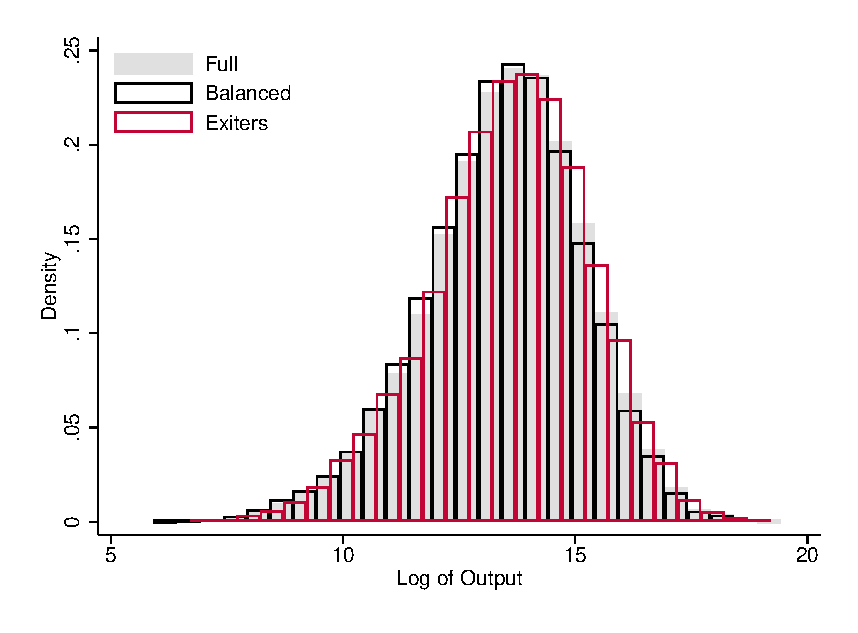
\includegraphics[width=\textwidth]{./histY.eps}
		\end{subfigure}
		\begin{subfigure}[b]{.495\textwidth}
			\centering
			\caption{Labor}
			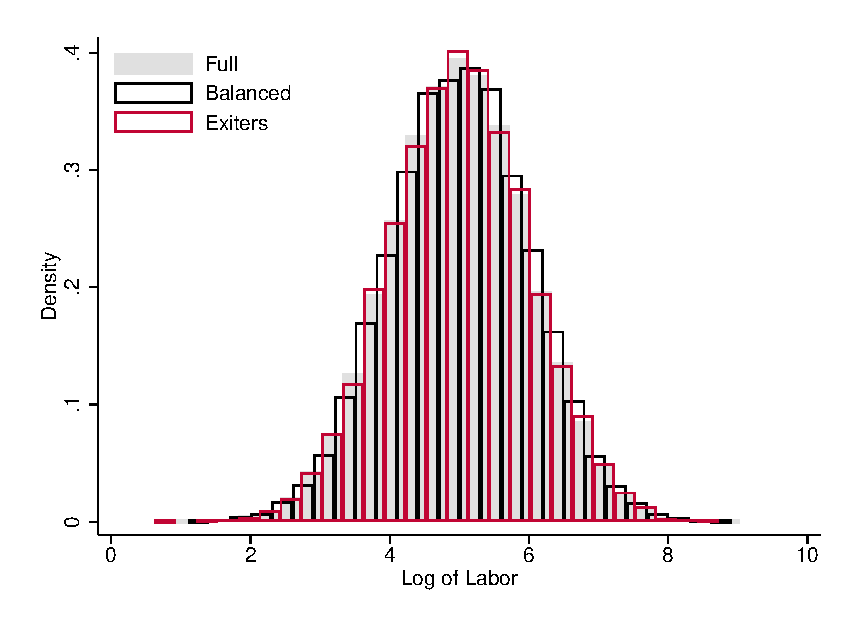
\includegraphics[width=\textwidth]{./histL.eps}
		\end{subfigure}\\
		\begin{subfigure}[b]{.495\textwidth}
			\centering
			\caption{Capital}
			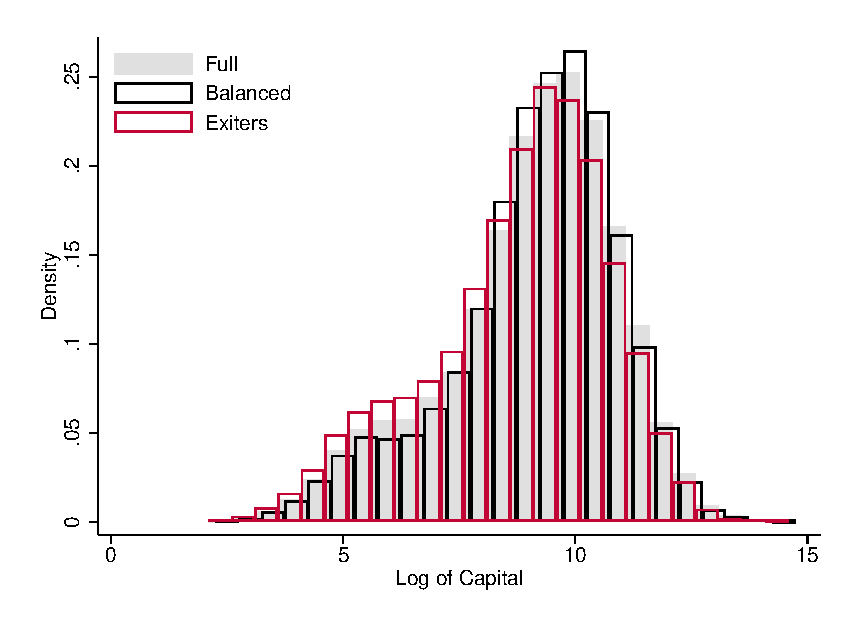
\includegraphics[width=\textwidth]{./histK.eps}
		\end{subfigure}
		\begin{subfigure}[b]{.495\textwidth}
			\centering
			\caption{Investment}
			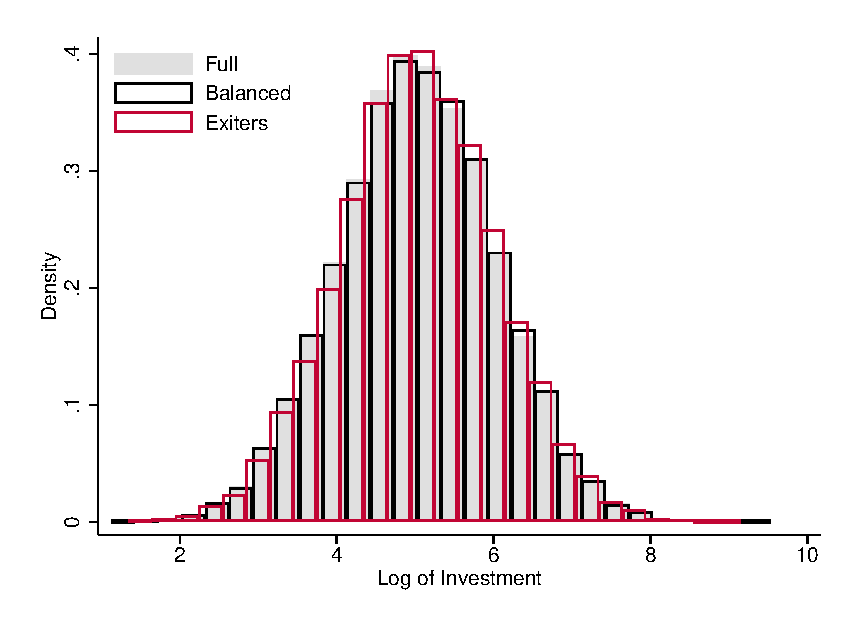
\includegraphics[width=\textwidth]{./histI.eps}
		\end{subfigure}
		
	\end{figure}
\end{comment}


\begin{figure}[ht]
	\caption{Time series by samples}\label{fig:time}
	\centering	
	\begin{subfigure}[b]{.3\textwidth}
		\centering
		\caption{Output}
		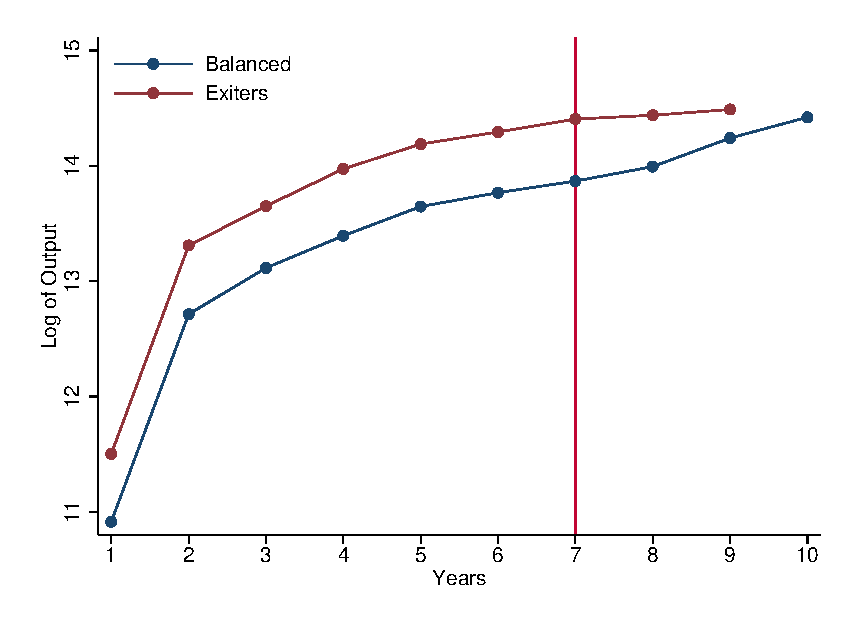
\includegraphics[width=\textwidth]{./timeY.eps}
	\end{subfigure}
	\begin{subfigure}[b]{.3\textwidth}
		\centering
		\caption{Labor}
		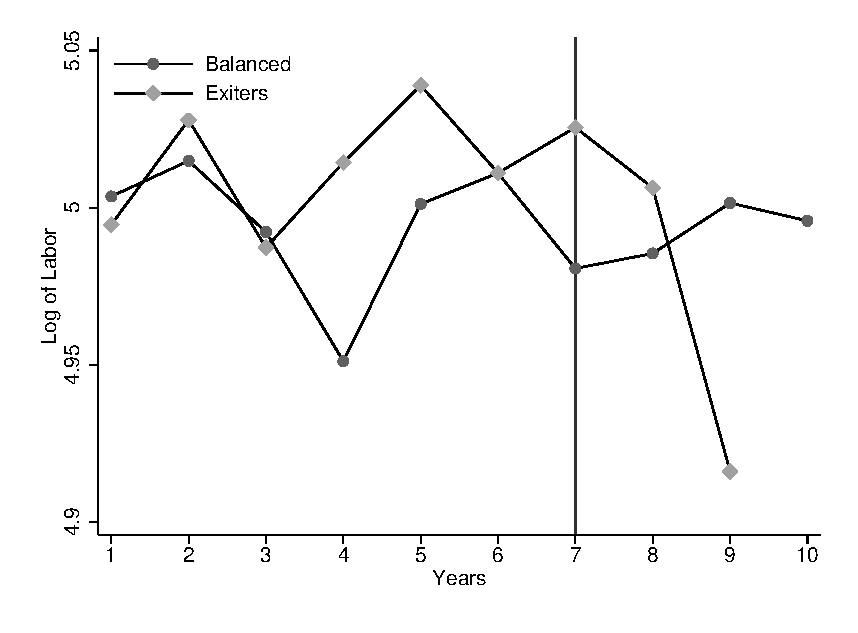
\includegraphics[width=\textwidth]{./timeL.eps}
	\end{subfigure}\\
	\begin{subfigure}[b]{.3\textwidth}
		\centering
		\caption{Capital}
		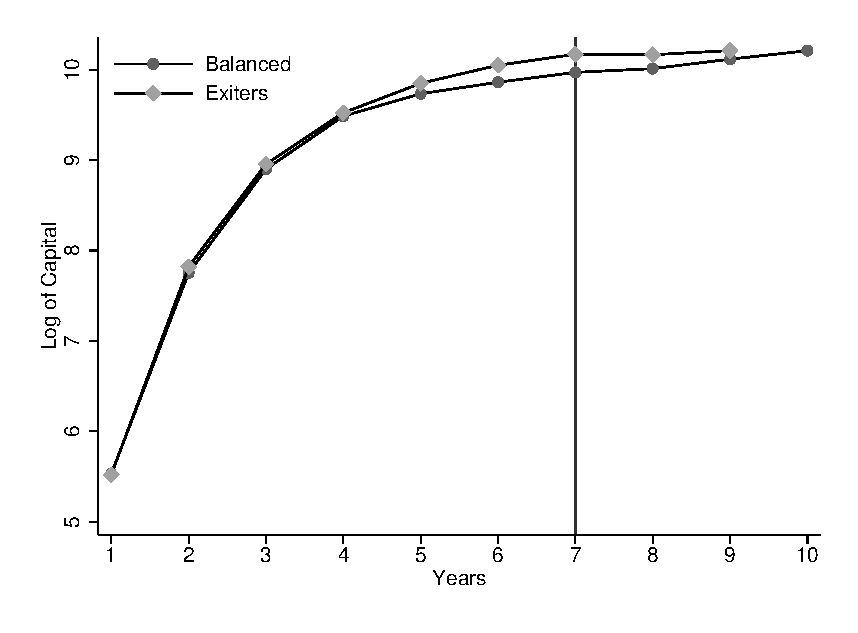
\includegraphics[width=\textwidth]{./timeK.eps}
	\end{subfigure}
	\begin{subfigure}[b]{.3\textwidth}
		\centering
		\caption{Investment}
		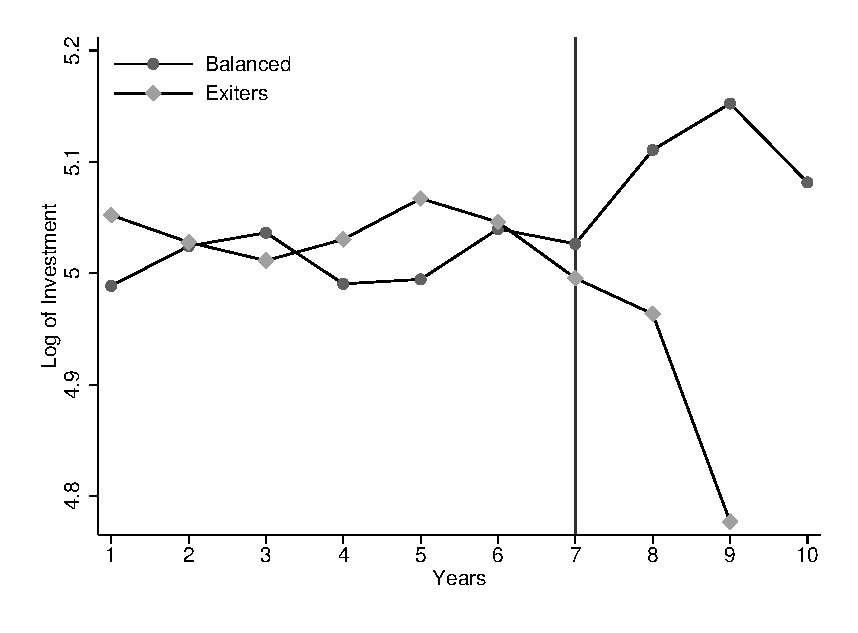
\includegraphics[width=\textwidth]{./timeI.eps}
	\end{subfigure}
\begin{tabular*}{1\textwidth}{c}
	\multicolumn{1}{p{1\hsize}}{\footnotesize Time series of average by year for both exiteres and firms that stay. Half of the exiters leave the market after year 7.}\\
\end{tabular*}      	  
\end{figure}

Firms that exit the market are, on average, 2.7 years older than the firms that stay in the market. As can be seen in \autoref{tab:exitstats}, the differences in distribution suggests that firms that leave the market have less capital and investment, similar labor, and higher output. Lower capital points toward the fact that exiters had less protection against negative shocks. \\
The fact that exiting firms have higher output is puzzling. However, as can be seen in \autoref{fig:time}, after year three, exiter firms seem to have tried to compensate for a bad productivity draw by increasing labor and investment. However, this overspending drove them to leave the market.

\subsection*{Question 2}
In order to estimate technology from a production function, we need the best possible estimates of the $\beta$s in the main regression because everything that we don't accurately account for in terms of labor, capital, and firm age will go in the error which will ultimately be the estimate of technology. We expect the labor coefficient to be positively biased given the simultaneity between a flexible input and output. Regarding capital, we expect it to suffer from both attenuation bias and negative bias. First, because of capital measurement error. Second, because of selection, since we are focused solely on the firms that stay which are the ones that have more capital and therefore have a lower productivity cutoff-level.\\

The results for the pooled, fixed, random, and between effects are shown in \autoref{tab:q2}. As can be seen in column (1), it is the case that the coefficient of labor is larger than the standard 0.3 in the US literature. Likewise, capital seems less that then benchmark of 0.6. However, it is important to note that the labor coefficient doesn't change much across specifications. \\

In the case of the within estimator (column (3)), we assume that the errors have the form $\varepsilon_{it}=\omega_i+\eta_{it}$. So if, for example, more productive firms hire more people, the fixed effect estimator is a better choice and should alleviate the positive bias for labor. However, it does not look like this is the case. The labor coefficient barely changes from the pooled estimator and the capital coefficient (which should be negatively biased because of selection) even decreases. Finally, only 13\% of the estimated variance is due to firm-level fixed effects, which points toward the fact that the within estimator is not addressing our main concerns. \\

Given that we suspect that the capital coefficient is both negatively biased and attenuated, the between model might be a better choice. The estimator for $\beta_k$ in the between model (column (2)) is the highest of all the regressions. \\

Finally, the Hausman test tell us that we can reject the null of the random and fixed effect estimators being statistically equivalent. The necessary asumption for random effects is very implausible in this setting because we precisely expect a non-zero correlation between the observed and unobserved variables. It is then not surprising that random effects estimators are almost the same as the pooled regression.


\begin{table}[htbp]\centering
\def\sym#1{\ifmmode^{#1}\else\(^{#1}\)\fi}
\caption{Total, Between, Within and Random Effects Estimators \label{tab:q2}}
\begin{tabular}{l*{4}{c}}
\toprule
                    &\multicolumn{1}{c}{(1)}&\multicolumn{1}{c}{(2)}&\multicolumn{1}{c}{(3)}&\multicolumn{1}{c}{(4)}\\
                    &\multicolumn{1}{c}{Pooled}&\multicolumn{1}{c}{Between}&\multicolumn{1}{c}{Within}&\multicolumn{1}{c}{Random Effects}\\
\midrule
Age of the firm     &       0.133\sym{***}&       0.128\sym{***}&       0.188\sym{***}&       0.133\sym{***}\\
                    &     (0.005)         &     (0.006)         &     (0.006)         &     (0.006)         \\
\addlinespace
Log of Capital      &       0.431\sym{***}&       0.555\sym{***}&       0.388\sym{***}&       0.421\sym{***}\\
                    &     (0.007)         &     (0.016)         &     (0.008)         &     (0.007)         \\
\addlinespace
Log of Labor        &       0.594\sym{***}&       0.613\sym{***}&       0.592\sym{***}&       0.594\sym{***}\\
                    &     (0.008)         &     (0.030)         &     (0.008)         &     (0.008)         \\
\midrule
Observations        &       21800         &       21800         &       21800         &       21800         \\
\bottomrule
\end{tabular}
\end{table}

\FloatBarrier

\subsection*{Question 3}

\begin{table}[htbp]\centering
\def\sym#1{\ifmmode^{#1}\else\(^{#1}\)\fi}
\caption{Difference Estimators \label{tab:q3}}
\begin{tabular}{l*{3}{c}}
\toprule
                    &\multicolumn{1}{c}{(1)}&\multicolumn{1}{c}{(2)}&\multicolumn{1}{c}{(3)}\\
                    &\multicolumn{1}{c}{First}&\multicolumn{1}{c}{Second}&\multicolumn{1}{c}{Third}\\
\midrule
Age of the firm     &       0.139\sym{***}&       0.101\sym{***}&       0.183\sym{***}\\
                    &     (0.013)         &     (0.009)         &     (0.008)         \\
\addlinespace
Log of Capital      &       0.252\sym{***}&       0.372\sym{***}&       0.399\sym{***}\\
                    &     (0.011)         &     (0.009)         &     (0.009)         \\
\addlinespace
Log of Labor        &       0.593\sym{***}&       0.595\sym{***}&       0.573\sym{***}\\
                    &     (0.009)         &     (0.009)         &     (0.009)         \\
\midrule
Observations        &       15260         &       15260         &       15260         \\
\bottomrule
\end{tabular}
\end{table}

\FloatBarrier

Taking the difference between time periods and running the regression on the differenced variables would only address our biases if we assume again that $\varepsilon_{it}=\omega_i+\eta_{it}$. In this scenario, the $\omega_i$ cancels out when we take the difference. There are two issue here. First, as we discussed above, this assumption on the structure of the errors is probably not right. Second, if the error term in measurement of capital varies in time, it is not canceled out by differencing the variables. Say true capital, $k^*_t$ has measurement error, then $k^*_{it}=k_{it}+\nu_{it}$. As we showed in class, this implies that the error term of the regression is $\eta_{it}^*-\beta_k\nu_{it}$. In this case, when we take first differences we get


\begin{align}\label{eq:bias}
 Cov(\Delta k_{it},\Delta \varepsilon_{it})& =
Cov\left(\Delta (k_{it}^*+\nu_{it} ),\Delta (\eta_{it}^*-\beta_k\nu_{it})\right) \quad \text{where $\Delta k_{it}=k_{it}-k_{ij}$ with $j<t$}\\ \nonumber
&=-\beta_k Var(\Delta \nu_{it})=-\beta_k Var(\nu_{it}-\nu_{it-1})\\ \nonumber
 &=-2\beta_k Var(\sigma^2_{\nu}-\rho_{t,j}) \quad \text{where $\rho_{t,j}$ is the serial correlation of $\nu$ between time $t$ and $j$}\\ \nonumber
 & 	\Rightarrow \ 
 plim(\hat{\beta_k})-\beta_k= -\frac{2(\sigma^2_{\nu}-\rho_{t,j})}{\sigma_{k}^2 } \\ \nonumber
\end{align}

The fact that the coefficient for capital in the pooled regression (\autoref{tab:q2}, column 1) is attenuated comes from the fact that the errors include the $-\beta_k\nu_{it}$ term from measurement error, so the estimator is biased towards zero. In column (1) of \autoref{tab:q3} the capital coefficient is even more attenuated now because the measurement error is amplified by the difference estimator. In columns (2)-(4), we can see that the capital coefficient increases as $\rho_{t,j}$ decreases (bigger time difference) because the bias from \autoref{eq:bias} is becoming smaller. These results show that running the difference regression, even up to three periods apart, only amplifies the bias from measurement error in capital. 


\subsection*{Question 4}
\subsubsection*{(a)}
\begin{table}[htbp]\centering
\def\sym#1{\ifmmode^{#1}\else\(^{#1}\)\fi}
\caption{Total and Within Estimators for Full Sample}
\begin{tabular}{l*{2}{c}}
\toprule
                    &\multicolumn{1}{c}{(1)}&\multicolumn{1}{c}{(2)}\\
                    &\multicolumn{1}{c}{Pooled}&\multicolumn{1}{c}{Within}\\
\midrule
Age of the firm     &       0.133\sym{***}&       0.198\sym{***}\\
                    &     (0.002)         &     (0.005)         \\
\addlinespace
Log of Capital      &       0.414\sym{***}&       0.362\sym{***}\\
                    &     (0.005)         &     (0.006)         \\
\addlinespace
Log of Labor        &       0.597\sym{***}&       0.594\sym{***}\\
                    &     (0.006)         &     (0.006)         \\
\midrule
Observations        &       39569         &       39569         \\
\bottomrule
\end{tabular}
\end{table}

\FloatBarrier

\subsubsection*{(b)}
\begin{table}[htbp]\centering
\def\sym#1{\ifmmode^{#1}\else\(^{#1}\)\fi}
\caption{Probit Model for Exiting Probability}
\begin{tabular}{l*{1}{c}}
\toprule
                    &\multicolumn{1}{c}{(1)}\\
                    &\multicolumn{1}{c}{Continuation Dummy}\\
\midrule
Log of Investment   &       0.477\sym{***}\\
                    &     (0.015)         \\
\addlinespace
Age of the firm     &      -0.692\sym{***}\\
                    &     (0.012)         \\
\addlinespace
Log of Capital      &       0.196\sym{***}\\
                    &     (0.011)         \\
\midrule
Observations        &       39569         \\
\bottomrule
\end{tabular}
\end{table}

\begin{table}[htbp]\centering
\def\sym#1{\ifmmode^{#1}\else\(^{#1}\)\fi}
\caption{Total and Within Estimators correcting for Selection}
\begin{tabular}{l*{2}{c}}
\toprule
                    &\multicolumn{1}{c}{(1)}&\multicolumn{1}{c}{(2)}\\
                    &\multicolumn{1}{c}{Pooled}&\multicolumn{1}{c}{Within}\\
\midrule
Age of the firm     &       0.130\sym{***}&       0.199\sym{***}\\
                    &     (0.003)         &     (0.005)         \\
\addlinespace
Log of Capital      &       0.415\sym{***}&       0.363\sym{***}\\
                    &     (0.005)         &     (0.006)         \\
\addlinespace
Log of Labor        &       0.597\sym{***}&       0.594\sym{***}\\
                    &     (0.006)         &     (0.006)         \\
\midrule
Observations        &       39569         &       39569         \\
\bottomrule
\end{tabular}
\end{table}

\FloatBarrier

\subsection*{Question 5}
\subsubsection*{(a)}
\begin{table}[htbp]\centering
\def\sym#1{\ifmmode^{#1}\else\(^{#1}\)\fi}
\caption{OP First Stage \label{tab:q5a}}
\begin{tabular}{l*{1}{c}}
\toprule
                    &\multicolumn{1}{c}{(1)}         \\
\midrule
Log of Labor        &       0.598\sym{***}\\
                    &     (0.006)         \\
\midrule
N                   &      39,569         \\
\bottomrule
\end{tabular}
\end{table}

\FloatBarrier
The coefficient obtained for labor here is similar to the one obtained in the question above, suggesting that endogeneity might not be such a big concern. 

\subsubsection*{(c)}
\begin{table}[htbp]\centering
\def\sym#1{\ifmmode^{#1}\else\(^{#1}\)\fi}
\caption{OP Second Stage \label{tab:q5c}}
\begin{tabular}{l*{1}{c}}
\toprule
                    &\multicolumn{1}{c}{(1)}         \\
\midrule
Log of Capital      &       0.271\sym{***}\\
                    &     (0.010)         \\
\addlinespace
Age of the firm     &       0.147\sym{***}\\
                    &     (0.006)         \\
\midrule
N                   &      34,672         \\
\bottomrule
\end{tabular}
\end{table}

\FloatBarrier
Comparing our results to the ones found in questions 2 and 4, we can see that the coefficient for capital (0.271) is lower than the one found in the all four specifications analyzed in question 2. The same applies to question 4. As expected, all coefficients are positive -- firms that suffer higher productivity shocks hire more capital. 
With respect to the coefficient for age of the firm (0.147), we verify the opposite. All coefficients found in questions 2 and 4 are lower for age than the one we found in the second-stage, but the differences are not as stark as for the capital case. 
This seems to suggest that endogeneity is a concern for the coefficient of capital. In addition, this model should also correct for measurement error.  
\newpage
\subsubsection*{(d)}
\begin{table}[htbp]\centering
\def\sym#1{\ifmmode^{#1}\else\(^{#1}\)\fi}
\caption{OP Second Stage correcting for Selection \label{tab:q5d}}
\begin{tabular}{l*{1}{c}}
\toprule
                    &\multicolumn{1}{c}{(1)}         \\
\midrule
Log of Capital      &       0.303\sym{***}\\
                    &     (0.013)         \\
\addlinespace
Age of the firm     &       0.113\sym{***}\\
                    &     (0.006)         \\
\midrule
N                   &      34,672         \\
\bottomrule
\end{tabular}
\end{table}

\FloatBarrier
After correcting for selection, our coefficient for capital rises, while the one for age decreases. 
This result makes sense, as selection should lead to a negative bias in the capital coefficient. 
\subsubsection*{(e)}
\begin{comment}
	\begin{table}[htbp]\centering
\def\sym#1{\ifmmode^{#1}\else\(^{#1}\)\fi}
\caption{OP Estimation correcting for Endogeneity and Selection \label{tab:q5e}}
\begin{tabular}{l*{1}{c}}
\toprule
                    &\multicolumn{1}{c}{(1)}\\
                    &\multicolumn{1}{c}{} \\
\midrule
Age of the firm     &       0.117\sym{***}\\
                    &     (0.007)         \\
\addlinespace
Log of Capital      &       0.292\sym{***}\\
                    &     (0.011)         \\
\addlinespace
Log of Labor        &       0.598\sym{***}\\
                    &     (0.006)         \\
\midrule
N                   &      39,569         \\
\bottomrule
\end{tabular}
\end{table}

\end{comment}
\FloatBarrier

The results are very similar to what was found before. The steps we went through before were simply a decomposition of this command.  



\end{document}